\documentclass[]{article}  % list options between brackets
\usepackage{}              % list packages between braces
\usepackage{mathptmx}
\usepackage{algorithm}
\usepackage{algorithmic}
\usepackage{graphicx}
\usepackage{cite}
\oddsidemargin  0.6in
\evensidemargin 0.6in

% type user-defined commands here

\begin{document}


\begin{figure}
	\centering
	  %\vspace{-4in}
		\includegraphics[width=4in]{figure/OgreHead.eps}
	%\caption{\small Shadow maps used to produce both cast shadows and self-shadows.}
	\label{OgreHead}
\end{figure}


\title{Shadow Mapping in Ogre}   % type title between braces
\author{\small Hamilton Chong}         % type author(s) between braces
\date{\small Aug 2006}    % type date between braces
\maketitle

\newpage

\begin{abstract}
A discussion of shadow mapping: the algorithm, variants, theory and analysis, and implementation.
\end{abstract}

\section{Introduction to the Shadow Mapping Algorithm}            
\label{Introduction}


Shadow mapping, an algorithm introduced by Lance Williams ~\cite{WIL78} and now prevalent in real-time and off-line rendering, is based on a simple idea:  First, a snapshot of the scene is taken from the viewpoint of the light.  Then, when creating an image from the perspective of the camera, the light's snapshot is used to determine visibility.  Parts of the scene seen by both the light and the camera must be lit (by the light in question).  Parts of the scene visible only to the camera must be shadowed.  We do not care about parts of the scene seen only by the light.  

In practice, the snapshot from the viewpoint of the light is stored as a floating point depth buffer.  It is important to use a format that supports enough precision to avoid shadow acne (z-fighting) on lit surfaces.  In Ogre, we can specify the depth format to use; in the example code, we will choose the 32-bit format. 

Once shadow determination has occurred (whether a fragment is in shadow or not), Ogre provides two different ways to render the shadows into the final image.  The modulative technique will uniformly darken regions of the image determined to be in shadow.  This is a cheaper and less accurate lighting model.  For instance, specular highlights in shadow will appear as darkened specular highlights.  The other technique is additive light masking.  This technique builds up contributions from each light in non-shadowed areas and adds them together to create the final image.  The code in section \ref{Implementation} will use additive light masking, but could just as easily be adapted for modulative shadows.

\subsection{Formalism}

Mathematically, the process can be represented as follows: Let $P_l$ and $P_c$ be the projection matrices for the light and camera respectively.  Let $M_l$ and $M_c$ be the modelview matrices for the light and camera coordinate systems.  Let $\vec{x} = [x_1,x_2,x_3,1]^t$ be a point in object space, $\vec{y} = [y_1,y_2,y_3,1]^t$ the screen space coordinates, and $\vec{u} = [u_1,u_2,u_3,1]^t$ the shadow map coordinates.  

\begin{eqnarray}
\label{eqn:hom}
    \left[ \begin{array}{c}
		u_1  w_l \\
		u_2  w_l \\
		u_3  w_l \\
		w_l     \end{array} \right] =  P_l M_l \left[ \begin{array}{c}
		x_1 \\
		x_2 \\
		x_3 \\
		1     \end{array} \right]
\end{eqnarray}

\begin{eqnarray}
\label{eqn:hom}
    \left[ \begin{array}{c}
		y_1  w_c \\
		y_2  w_c \\
		y_3  w_c \\
		w_c     \end{array} \right] =  P_c M_c \left[ \begin{array}{c}
		x_1 \\
		x_2 \\
		x_3 \\
		1     \end{array} \right]
\end{eqnarray}

These equations can be written more concisely as: $\vec{u}w_l = P_l M_l \vec{x}$ and $\vec{y} w_c = P_c M_c \vec{x}$.  Division of $\vec{u}w_l$ and $\vec{y}w_c$ by their respective homogeneous coordinates yields the Euclidean representations $\vec{u}$ and $\vec{y}$.

Note that while $P_c$ and $M_c$ are completely determined by the camera image we want to produce, we have some ambiguity in the $P_l$ and $M_l$ chosen for shadow mapping.  The degrees of freedom here are later exploited to combat the aliasing issue.  

\subsection{Depth Biasing}
\label{DepthBias}

\begin{figure}
	\centering
	  \vspace{-0.8in}
	  \hspace{-0.8in}
		\includegraphics[width=3in]{figure/depthbias.eps}
	\vspace{-1in}
	\caption{\em \small Shadow map sample must use one float to represent a range of possible depth values.  A depth sample is chosen in the middle.  Any camera image point in between the two camera rays will see the geometry, and depending on distance from light will report differently on shadowed versus lit.  However, every such point should be lit.}
	\label{fig:bias}
\end{figure}

Due to the finite precision of floating point representations and inherent inability of one number to represent a range of values, it is often necessary to add a little bias to the depth values stored in a shadow map.  One does not simply store the $u_3$ value.  Figure \ref{fig:bias} illustrates the issue.  Here we have used blue dots on the light's image plane to represent boundaries between shadow ``texels.''  The interval in between the dots then represents a shadow map sample for which a single depth value (float) is stored.  For the sample whose boundary rays are shown, the red dot's depth is saved.  However, note that from the camera's perspective, any (camera) image point in between the two drawn camera rays will hit the scene geometry within the shadow map sample's interval.  Hence, the same shadow map sample depth will be used to determine visibility for all such camera pixels.  Camera pixels whose rays fall to the right of the red dot will be marked as shadowed, while pixels whose rays fall to the left of the red dot will be marked as lit.  This is not the right behavior because clearly all the pixels should be marked as lit.  As we can see, a depth bias is needed.  By pushing the shadow map sample's depth farther (to the 2nd red dot), we can achieve correct shadow determination.  

One could approach the depth bias issue in a completely {\em ad hoc} manner, but it is possible to do better.  One would ideally compute a bias that depends on how depth ($u_3$) changes between shadow map samples.  The change in depth as one moves a unit step (to the next shadow map sample) represents the ambiguity of the depth value.  Such a value may seem intractable to compute, but calculus and linear algebra save the day.  From calculus, we learn that the derivative provides the best linear approximation to any function ($u_3 = u_3(u_1, u_2)$ in particular).  In multiple dimensions, this role is played by the Jacobian (matrix of partial derivatives).  In other words, we want to compute $\frac{du_3}{du_1}$ and $\frac{du_3}{du_2}$, where we have treated $u_3$ as a function of $u_1$ and $u_2$.  Once these values are computed, it makes sense to then add some weighted combination of these to the stored depth value (e.g., some scale of the Jacobian's Frobenius norm).  

But even if the light is staring at a plane straight on (view direciton lines up with plane's normal), making $\frac{du_3}{du_1}$ and $\frac{du_3}{du_2}$ both zero, we would still need a slight offset because rounding due to the float's finite representation may still cause shadow acne.  In this case, we'd like to offset the depth by a small value that pushes it beyond rounding ambiguity.  While one could use an arbitrary constant offset, this is unsatisfactory since the constant in light image space corresponds to varying amounts of offset in light space (pre-projection Euclidean space with light's position at origin).  Let us instead choose a constant offset in the z direction of {\em light space} and compute what the offset for a particular sample should be in {\em light image space}.  In Ogre's example code, the small constant offset in light space is chosen to be 1 unit.  If 1 is not a small amount in your engine's chosen scale, you can easily change this choice.  At any rate, the relevant quantity is $\frac{\partial u_3}{\partial X_3}$ where $\vec{X} = M_l \vec{x}$.

The choices here closely mirror what OpenGL implements through glPolygonOffset.  The second adjustment is slightly different since OpenGL chooses a vendor specific fudge factor.  

Equations for computing the stated quantities are provided below.  One need not wade through these to use the depth biasing code.  Understanding what the relevant parameters explained above are (in case adjustment is needed) is sufficient.

\begin{eqnarray}  
\label{eqn:dxqdu}
  \frac{\partial (\vec{x} q_l)}{\partial u_i} = \mbox{i-th column of } M_l^{-1} P_l^{-1} V_l^{-1} 
\end{eqnarray}
where $V_l$ is the viewport matrix for the light and $i=1,2,3$.  $q_l$ turns out to be $1/w_l$.

\begin{eqnarray} 
\label{eqn:dxdu}
  \frac{\partial \vec{x}}{\partial u_i} = \frac{1}{q_l} \left( \frac{\partial (\vec{x} q_l)}{\partial u_i} - \vec{x}\frac{\partial q_l}{\partial u_i} \right) \\
\label{eqn:du3du}
  \frac{du_3}{du_j} = \left( \vec{n} \cdot \frac{\partial \vec{x}}{\partial u_3} \right)^{-1} \left( \vec{n} \cdot \frac{\partial \vec{x}}{\partial u_j} \right)
\end{eqnarray}
where $\vec{n}$ is the normal at point $\vec{x}$ and $j=1,2$.  Note that (\ref{eqn:du3du}) is exactly the set of values needed for the first part.


\begin{eqnarray}  
\label{eqn:duwdX3}
  \frac{\partial (\vec{u} w_l)}{\partial X_3} = \mbox{3rd column of } P_l \\
\label{eqn:dudX3}
  \frac{\partial \vec{u}}{\partial X_3} = \frac{1}{w_l} \left( \frac{\partial (\vec{u} w_l)}{\partial X_3} - \vec{u}\frac{\partial w_l}{\partial X_3} \right)
\end{eqnarray}

Note that (\ref{eqn:dudX3}) is the quantity needed for the second bias term.  This is also the term to scale for different choices of small offset in light space.  If 0.01 units is the small offset, scale this value by 0.01.  

\subsection{Percentage Closest Filtering}
As widely known, shadow mapping can exhibit significant aliasing.  When this happens during texture mapping we apply filtering.  We'd like to apply a similar principle with shadow maps, but filtering depth values is categorically the wrong thing to do.  As described in ~\cite{RSC87}, one should instead filter depth test results.  This is termed percentage closest filtering.  Ideally this would be a filtering technique much like anisotropic texture filtering, but for simplicity and efficiency, Ogre's example code implements the bilinear analogue.

%-----------------------------------------------------------------------------------------------------

\section{Variants}

There are many shadow mapping variants.  Enumerating (much less describing) all of them would take us too far afield in this article.  We instead defer to the provided references and google for such coverage.  The many variants can, however, be broken up into three broad categories: (1) Those that store additional information beyond a single float, (2) those that divide up shadow frusta into multiple frusta to be handled separately, and (3) those that propose less naive $P_l$ and $M_l$ to use and thereby affect the sampling distribution.  Algorithms in each category usually work quite independently and so many hybrid approaches are easily conceivable.  

\subsection{Storing Additional Info}
One example of this is Deep Shadow Maps ~\cite{LV00}.  In this work, instead of storing a single depth value and treating visibility as a binary value, a transfer function is stored and visibility is continuous.  This algorithm is important in offline movie rendering, but also relevant to the Variance Shadow Mapping algorithm elucidated by the game developer community ~\cite{DL06}.  

While variance shadow maps are motivated by statistical considerations, it is perhaps more properly understood in the Deep Shadow Maps framework.  Analyzing it in terms of distributions is flawed for two reasons: (1) the inequality considered is valid only for unimodal distributions whereas depth values are often discontinuous in regions that matter; (2) the inequality is treated as equality.  The equations are justified with a very specific example in which two planes are viewed straight on.  In practice there are very noticeable halo effects around objects, which makes more heuristic tweaks necessary.

Recasting this into the framework of deep shadow maps, we see that the proposed equality is simply a particular functional approximation to the transfer function.  Variance shadow maps proposes a two-parameter family of approximation functions whose parameters are linearly interpolated in the usual way.  This viewpoint allows for analysis and also suggests the possibility of getting improvements via other approximating functional forms.  

\subsection{Breaking up Shadow Frusta}

Adaptive Shadow Maps ~\cite{FFB01} are an example of this.  It is still largely considered too expensive for real-time rendering, but continued research and growing GPU power may make some variant worthwhile.  

\subsection{Playing with Projection Matrices}
\label{sect:planeopt}
There are various heuristic approaches for choosing $P_l$ and $M_l$, but here we will focus on one method, the Plane Optimal algorithm ~\cite{Chong04}, that provides a particular guarantee.  For this algorithm, we specify a plane of interest (e.g., ground plane, wall, table top) for which we want perfect shadowing no matter the configuration of light and camera in the scene (even dueling frusta).  The algorithm will then compute $P_l$ and $M_l$ so that the mapping between camera image and light image is the identity when restricted to the plane.  If the shadow map matches the resolution of the screen, then each pixel gets exactly one shadow sample.  Shadows off the plane of interest have no guarantees.  
One limitation of the method is shown in Figure \ref{fig:planeopt}.  Only region I will be shadowed and self-shadowed properly, with points on the plane being shadowed perfectly (alias-free).  This makes the method perhaps most useful for games where the view is top-down or isometric (like RTS games).  It is also useful for cases like dueling frusta (where just about all other methods fail).  

\begin{figure}
	\centering
	  \vspace{-0.8in}
	  \hspace{-0.8in}
		\includegraphics[width=3in]{figure/optfrust.eps}
	\vspace{-1in}
	\caption{\em \small Region I is defined as the set of all points along rays between the light and a point on the plane of interest in the camera's view.  Everything in region I is shadowed and self-shadowed properly.  Objects in region II are not self-shadowed properly.}
	\label{fig:planeopt}
\end{figure}


\section{Theory and Analysis}
A full discussion of shadow map analysis is beyond the scope of this article.  For those interested, the references ~\cite{Chong06} and ~\cite{Chong04} are good (in my extremely biased opinion).  Note that as research papers, they are quite concise.  Unfortunately there don't seem to more step-by-step expositions available at this moment.  

There has been a lot of academic and industry research on improving shadow maps.  However, analyses presented on shadow maps often do not say what people claim they say.  These faulty conclusions usually come from considering very special cases and assuming the general case is very similar.  For clarification, we explore some of these misconceptions here.  

\subsection{(Non)Optimality of Logarithmic Shadow Maps}
We start with one {\em heuristic} that has gained quite a bit of traction: the idea of using some logarithmic mapping between light space and light image space instead of a projective transform.  A number of algorithms based on this idea have been proposed, and even some hardware changes.  Much of this work seems to be motivated by the incorrect assumption that logarithmic mappings are optimal.  

The very special motivating case is this:  The camera looks down the z axis.  Directional light illuminates the scene perpendicular to the z axis.  An angled piece of a plane is viewed by the camera.  As the angled piece of plane is pulled along the camera ray direction, using a logarithmic shadow map gives us constant shadow quality on this geometric piece.  But unless we're rendering translucent dust particles along a camera ray, this analysis is irrelevant.  If the dust particles are not translucent, we only care about shadow determination on the first one, not a whole line of them.  If we are rendering continuous surfaces (resp. curves), we care about the quality as one moves in the tangent plane (resp. tangent) direction because this is the best linear approximation to the surface (resp. curve), not the camera ray direction.  

In fact, in the case of a chosen plane of interest for example, we know we can get completely alias free shadow mapping using a projective transform (section \ref{sect:planeopt}).  Logarithmic shadow maps may be an interesting heuristic to try out, but certainly not worth changing hardware over in my opinion.  If you're going to change hardware, might as well aim for true optimality.  

\subsection{Sampling Aliasing versus Depth Precision Aliasing}
Sometimes people tend to conflate these two sources of aliasing.  They note that after applying some sort of custom projective transform, the depth values are warped as well.  This problem can be completely overcome via the depth replacement method prescribed in Trapezoidal Shadow Maps ~\cite{MT04}.  So this is a completely orthogonal issue.  Depth precision can be just as good as ``normal'' shadow maps, no matter the perspective warp used to affect sampling.  

\subsection{Projective versus Perspective Aliasing}
The terms perspective and projective aliasing appeared in the Perspective Shadow Maps ~\cite{SD02} paper and has since been used extensively by those who work on improving shadow heuristics.  Often it is claimed that methods ameliorate perspective aliasing while projective aliasing is either unavoidable or must be addressed via completely separate means.  However, the distinction between the two is somewhat artificial.  Both result from not allocating enough shadow map samples to regions that matter to the viewer.  As the Plane Optimal algorithm demonstrates, it is possible to completely remove projective aliasing (as well as perspective aliasing) in certain scenes.  In general, there should be one combined measure of aliasing and algorithms must minimize this quantity.  See ~\cite{Chong06} for a unified notion of aliasing.  


\section{Implementation}
\label{Implementation}

Ogre provides a powerful framework that allows us to do a lot of shadow map customization.  
In Ogre, we turn on custom shadow mapping through the scene manager (here, sceneMgr).  It is recommended that this happen early as it may affect how certain resources are loaded.  

\begin{verbatim}
  // Use Ogre's custom shadow mapping ability
	sceneMgr->setShadowTexturePixelFormat(PF_FLOAT32_R);
	sceneMgr->setShadowTechnique( SHADOWTYPE_TEXTURE_ADDITIVE );
	sceneMgr->setShadowTextureCasterMaterial("CustomShadows/ShadowCaster");
	sceneMgr->setShadowTextureReceiverMaterial("CustomShadows/ShadowReceiver");
	sceneMgr->setShadowTextureSelfShadow(true);	
	sceneMgr->setShadowTextureSize(512);
\end{verbatim}

The setShadowTechnique call is all that is required for Ogre's default shadow mapping.  
In the code above, we have told Ogre to use the R channel of a floating point texture to store depth values.  This tends to be a very portable method (over graphics cards and APIs).  The sample sticks to using Ogre's default of 512x512 shadow maps.  Self-shadowing is turned on, but be warned that this will only work properly if appropriate depth biasing is also used.  The example code will manually account for depth biasing via the method described above in section \ref{DepthBias}.  The shadow caster and shadow receiver materials are defined in a materials script.  They tell Ogre which shaders to use when rendering shadow casters into the shadow map and rendering shadow receivers during shadow determination.  

The CustomShadows.material material script is given below:
\begin{verbatim}
// Shadow Caster __________________________________________________


vertex_program CustomShadows/ShadowCasterVP/Cg cg
{
    source customshadowcastervp.cg
    entry_point main
    profiles arbvp1 vs_2_0

    default_params
    {
        param_named_auto uModelViewProjection worldviewproj_matrix
    }
}

fragment_program CustomShadows/ShadowCasterFP/Cg cg
{
    source customshadowcasterfp.cg
    entry_point main
    profiles arbfp1 ps_2_0

    default_params
    {
        param_named      uDepthOffset float       1.0
        param_named      uSTexWidth float         512.0
        param_named      uSTexHeight float        512.0
        param_named_auto uInvModelViewProjection  inverse_worldviewproj_matrix
        param_named_auto uProjection              projection_matrix
    }
}

vertex_program CustomShadows/ShadowCasterVP/GLSL glsl
{
    source customshadowcastervp.vert

    default_params
    {
        param_named_auto uModelViewProjection worldviewproj_matrix
    }
}

fragment_program CustomShadows/ShadowCasterFP/GLSL glsl
{
    source customshadowcasterfp.frag

    default_params
    {
        param_named      uDepthOffset float       1.0
        param_named      uSTexWidth float         512.0
        param_named      uSTexHeight float        512.0
        param_named_auto uInvModelViewProjection  inverse_worldviewproj_matrix
        param_named_auto uProjection              projection_matrix
    }
}

vertex_program CustomShadows/ShadowCasterVP/HLSL hlsl
{
    source customshadowcastervp.hlsl
    entry_point main
    target vs_2_0

    default_params
    {
        param_named_auto uModelViewProjection worldviewproj_matrix
    }
}

fragment_program CustomShadows/ShadowCasterFP/HLSL hlsl
{
    source customshadowcasterfp.hlsl
    entry_point main
    target ps_2_0

    default_params
    {
        param_named      uDepthOffset float       1.0
        param_named      uSTexWidth float         512.0
        param_named      uSTexHeight float        512.0
        param_named_auto uInvModelViewProjection  inverse_worldviewproj_matrix
        param_named_auto uProjection              projection_matrix
    }
}

material CustomShadows/ShadowCaster
{
    technique glsl
    {
        // Z-write only pass
        pass Z-write
        {
            vertex_program_ref CustomShadows/ShadowCasterVP/GLSL
            {
            }
            fragment_program_ref CustomShadows/ShadowCasterFP/GLSL
            {
            }
        }
    }

    technique hlsl
    {
        // Z-write only pass
        pass Z-write
        {
            //Instead of using depth_bias, we'll be implementing it manually

            vertex_program_ref CustomShadows/ShadowCasterVP/HLSL
            {
            }
            fragment_program_ref CustomShadows/ShadowCasterFP/HLSL
            {
            }
        }
    }

	technique cg
    {
        // Z-write only pass
        pass Z-write
        {
            //Instead of using depth_bias, we'll be implementing it manually

            vertex_program_ref CustomShadows/ShadowCasterVP/Cg
            {
            }
            fragment_program_ref CustomShadows/ShadowCasterFP/Cg
            {
            }
        }
    }
}



// Shadow Receiver ________________________________________________

vertex_program CustomShadows/ShadowReceiverVP/Cg cg
{
    source customshadowreceivervp.cg
    entry_point main
    profiles arbvp1 vs_2_0

    default_params
    {
        param_named_auto uModelViewProjection   worldviewproj_matrix
        param_named_auto uLightPosition         light_position_object_space 0
        param_named_auto uModel                 world_matrix
        param_named_auto uTextureViewProjection texture_viewproj_matrix
    }
}

fragment_program CustomShadows/ShadowReceiverFP/Cg cg
{
    source customshadowreceiverfp.cg
    entry_point main
    profiles arbfp1 ps_2_x

    default_params
    {
        param_named uSTexWidth  float 512.0
        param_named uSTexHeight float 512.0
    }
}

vertex_program CustomShadows/ShadowReceiverVP/GLSL glsl
{
    source customshadowreceiver.vert
    
    default_params
    {
        param_named_auto uModelViewProjection   worldviewproj_matrix
        param_named_auto uLightPosition         light_position_object_space 0
        param_named_auto uModel                 world_matrix
        param_named_auto uTextureViewProjection texture_viewproj_matrix
    }
}

fragment_program CustomShadows/ShadowReceiverFP/GLSL glsl
{
    source customshadowreceiver.frag

    default_params
    {
        param_named uSTexWidth  float 512.0
        param_named uSTexHeight float 512.0
    }
}

vertex_program CustomShadows/ShadowReceiverVP/HLSL hlsl
{
    source customshadowreceivervp.hlsl
    entry_point main
    target vs_2_0

    default_params
    {
        param_named_auto uModelViewProjection   worldviewproj_matrix
        param_named_auto uLightPosition         light_position_object_space 0
        param_named_auto uModel                 world_matrix
        param_named_auto uTextureViewProjection texture_viewproj_matrix
    }
}

fragment_program CustomShadows/ShadowReceiverFP/HLSL hlsl
{
    source customshadowreceiverfp.hlsl
    entry_point main
    target ps_3_0

    default_params
    {
        param_named uSTexWidth  float 512.0
        param_named uSTexHeight float 512.0
    }
}

material CustomShadows/ShadowReceiver
{
    technique glsl
    {
        pass lighting
        {
            vertex_program_ref CustomShadows/ShadowReceiverVP/GLSL
            {
            }

            fragment_program_ref CustomShadows/ShadowReceiverFP/GLSL
            {
                param_named uShadowMap int 0
            }

            texture_unit ShadowMap
            {
                tex_address_mode clamp
                filtering none
            }
        }
    }

    technique hlsl
    {
        pass lighting
        {
            vertex_program_ref CustomShadows/ShadowReceiverVP/HLSL
            {
            }

            fragment_program_ref CustomShadows/ShadowReceiverFP/HLSL
            {
            }

            // we won't rely on hardware specific filtering of z-tests
            texture_unit ShadowMap
            {
                tex_address_mode clamp
                filtering none
            }
        }
    }

	technique cg
    {
        pass lighting
        {
            vertex_program_ref CustomShadows/ShadowReceiverVP/Cg
            {
            }

            fragment_program_ref CustomShadows/ShadowReceiverFP/Cg
            {
            }

            // we won't rely on hardware specific filtering of z-tests
            texture_unit ShadowMap
            {
                tex_address_mode clamp
                filtering none
            }
        }
    }
}
\end{verbatim}

Three techniques are presented, one for GLSL, one for HLSL, and one for Cg.  We'll present the GLSL code below.  Note that while most of the shader files are direct translations of each other, DirectX HLSL shaders must handle percentage closest filtering slightly differently from OpenGL.  OpenGL chooses the convention of having integers index sample centers whereas DirectX chooses integers to index sample corners.  Also note the variable names in the shaders presented below are slightly different from those presented earlier in this document.  This is due in part to the awkwardness of expressing subscripts in variable names and also in part because $u_3$ is less evocative of depth than $z$, etc.  With minimal effort one can match the shader equations with those presented earlier.  The code is presented here mostly to demonstrate how things fit together.  

\begin{verbatim}
//////////////////////////////////////////////////////////////////
//
// shadowcastervp.vert
//
// This is an example vertex shader for shadow caster objects.  
//
//////////////////////////////////////////////////////////////////


// I N P U T   V A R I A B L E S /////////////////////////////////

uniform mat4 uModelViewProjection;   // modelview projection matrix

// O U T P U T   V A R I A B L E S ///////////////////////////////

varying vec4 pPosition;      // post projection position coordinates
varying vec4 pNormal;        // normal in object space (to be interpolated)
varying vec4 pModelPos;      // position in object space (to be interpolated) 

// M A I N ///////////////////////////////////////////////////////

void main()
{
    // Transform vertex position into post projective (homogenous screen) space.
    gl_Position = uModelViewProjection * gl_Vertex;
    pPosition   = uModelViewProjection * gl_Vertex;
   
    // copy over data to interpolate using perspective correct interpolation
    pNormal   = vec4(gl_Normal.x, gl_Normal.y, gl_Normal.z, 0.0);
    pModelPos = gl_Vertex;
}
\end{verbatim}
This is a pretty standard vertex shader.

\begin{verbatim}
/////////////////////////////////////////////////////////////////////////////////
//
// shadowcasterfp.frag
//
// This is an example fragment shader for shadow caster objects.  
//
/////////////////////////////////////////////////////////////////////////////////

// I N P U T   V A R I A B L E S ////////////////////////////////////////////////

// uniform constants
uniform float uDepthOffset;           // offset amount (constant in eye space)
uniform float uSTexWidth;             // shadow map texture width
uniform float uSTexHeight;            // shadow map texture height
uniform mat4  uInvModelViewProjection;// inverse model-view-projection matrix
uniform mat4  uProjection;            // projection matrix

// per fragment inputs
varying vec4 pPosition;      // position of fragment (in homogeneous coordinates)
varying vec4 pNormal;        // un-normalized normal in object space
varying vec4 pModelPos;      // coordinates of model in object space at this point


// M A I N //////////////////////////////////////////////////////////////////////

void main(void)
{
    // compute the "normalized device coordinates" (no viewport applied yet)
    vec4 postProj = pPosition / pPosition.w;

    // get the normalized normal of the geometry seen at this point
    vec4 normal = normalize(pNormal);


    // -- Computing Depth Bias Quantities -----------------------------

    // We want to compute the "depth slope" of the polygon.  
    // This is the change in z value that accompanies a change in x or y on screen
    // such that the coordinates stay on the triangle. 
    // The depth slope, dzlen below, is a measure of the uncertainty in our z value 
    // Roughly, these equations come from re-arrangement of the product rule:
    // d(uq) = d(u)q + u d(q) --> d(u) = 1/q * (d(uq) - u d(q))
    vec4 duqdx = uInvModelViewProjection * vec4(1.0/uSTexWidth,0.0,0.0,0.0);
    vec4 dudx  = pPosition.w * (duqdx - (pModelPos * duqdx.w));
    vec4 duqdy = uInvModelViewProjection * vec4(0.0,1.0/uSTexHeight,0.0,0.0);
    vec4 dudy  = pPosition.w * (duqdy - (pModelPos * duqdy.w));
    vec4 duqdz = uInvModelViewProjection * vec4(0.0,0.0,1.0,0.0);
    vec4 dudz  = pPosition.w * (duqdz - (pModelPos * duqdz.w));
    // The next relations come from the requirement dot(normal, displacement) = 0
    float denom = 1.0 / dot(normal.xyz, dudz.xyz);
    vec2  dz = -  vec2( dot(normal.xyz, dudx.xyz) * denom , 
                         dot(normal.xyz, dudy.xyz) * denom );
    float  dzlen = max(abs(dz.x), abs(dz.y)); 


    // We now compute the change in z that would signify a push in the z direction
    // by 1 unit in eye space.  Note that eye space z is related in a nonlinear way to
    // screen space z, so this is not just a constant.  
    // ddepth below is how much screen space z at this point would change for that push.
    // NOTE: computation of ddepth likely differs from OpenGL's glPolygonOffset "unit"
    //  computation, which is allowed to be vendor specific.
    vec4 dpwdz = uProjection * vec4(0.0, 0.0, 1.0, 0.0);
    vec4 dpdz = (dpwdz - (postProj * dpwdz.w)) / pPosition.w;
    float  ddepth = abs(dpdz.z);

    // -- End depth bias helper section --------------------------------   

    // We now compute the depth of the fragment.  This is the actual depth value plus
    // our depth bias.  The depth bias depends on how uncertain we are about the z value
    // plus some constant push in the z direction.  The exact coefficients to use are
    // up to you, but at least it should be somewhat intuitive now what the tradeoffs are.
    float depthval = postProj.z + (0.5 * dzlen)+ (uDepthOffset * ddepth);
    depthval = (0.5 * depthval) + 0.5; // put into [0,1] range instead of [-1,1] 

    gl_FragColor = vec4(depthval, depthval, depthval, 0.0);
}
\end{verbatim}
This shader computes the two depth bias pieces described in section \ref{DepthBias}.  These are used to offset the stored depth value.  This is where the notation differs from above, but the translation is quite straightforward.

\begin{verbatim}
//////////////////////////////////////////////////////////////////
//
// shadowreceiver.vert
//
//////////////////////////////////////////////////////////////////


// I N P U T   V A R I A B L E S /////////////////////////////////

uniform mat4 uModelViewProjection;	// modelview projection matrix
uniform mat4 uModel;                    // model matrix
uniform mat4 uTextureViewProjection;    // shadow map's view projection matrix
uniform vec4 uLightPosition;            // light position in object space


// O U T P U T   V A R I A B L E S ///////////////////////////////

varying vec4   pShadowCoord;    // vertex position in shadow map coordinates
varying float  pDiffuse;        // diffuse shading value

// M A I N ///////////////////////////////////////////////////////

void main()
{
    // compute diffuse shading
    vec3 lightDirection = normalize(uLightPosition.xyz - gl_Vertex.xyz);
    pDiffuse = dot(gl_Normal.xyz, lightDirection);

    // compute shadow map lookup coordinates
    pShadowCoord = uTextureViewProjection * (uModel * gl_Vertex);

    // compute vertex's homogenous screen-space coordinates
    // Use following line if other passes use shaders
    //gl_Position = uModelViewProjection * gl_Vertex;	
    gl_Position = ftransform();	// uncomment if other passes use fixed function pipeline
}
\end{verbatim}
This is a pretty standard vertex shader as well.  The ftransform() function guarantees the output matches the fixed function pipeline.  If the objects you render use shaders instead of fixed function, then you should do so here as well.

\begin{verbatim}
/////////////////////////////////////////////////////////////////////////////////
//
// shadowreceiver.frag
//
/////////////////////////////////////////////////////////////////////////////////

// I N P U T   V A R I A B L E S ////////////////////////////////////////////////

// uniform constants
uniform sampler2D    uShadowMap;
uniform float        uSTexWidth;
uniform float        uSTexHeight;

// per fragment inputs
varying vec4   pShadowCoord;    // vertex position in shadow map coordinates
varying float  pDiffuse;        // diffuse shading value

// M A I N //////////////////////////////////////////////////////////////////////

void main(void)
{
    // compute the shadow coordinates for texture lookup
    // NOTE: texture_viewproj_matrix maps z into [0,1] range, not [-1,1], so
    //  have to make sure shadow caster stores depth values with same convention.
    vec4 scoord = pShadowCoord / pShadowCoord.w;


    // -- "Percentage Closest Filtering" ----------------------------------------- 

    // One could use scoord.xy to look up the shadow map for depth testing, but
    // we'll be implementing a simple "percentage closest filtering" algorithm instead.
    // This mimics the behavior of turning on bilinear filtering on NVIDIA hardware
    // when also performing shadow comparisons.  This causes bilinear filtering of
    // depth tests.  Note that this is NOT the same as bilinear filtering the depth
    // values and then doing the depth comparison.  The two operations are not 
    // commutative.  PCF is explicitly about filtering the test values since
    // testing filtered z values is often meaningless.  

    // Real percentage closest filtering should sample from the entire footprint
    // on the shadow map, not just seek the closest four sample points.  Such 
    // an improvement is for future work.

    
    // NOTE: Assuming OpenGL convention for texture lookups with integers in centers.
    //  DX convention is to have integers mark sample corners
    vec2 tcoord;
    tcoord.x = (scoord.x * uSTexWidth) - 0.5;
    tcoord.y = (scoord.y * uSTexHeight) - 0.5;
    float x0 = floor(tcoord.x);
    float x1 = ceil(tcoord.x);
    float fracx = fract(tcoord.x);
    float y0 = floor(tcoord.y);
    float y1 = ceil(tcoord.y);
    float fracy = fract(tcoord.y);
    
    // sample coordinates in [0,1]^2 domain
    vec2 t00, t01, t10, t11;
    float invWidth  = 1.0 / uSTexWidth;
    float invHeight = 1.0 / uSTexHeight;
    t00 = float2((x0+0.5) * invWidth, (y0+0.5) * invHeight);
    t10 = float2((x1+0.5) * invWidth, (y0+0.5) * invHeight);
    t01 = float2((x0+0.5) * invWidth, (y1+0.5) * invHeight);
    t11 = float2((x1+0.5) * invWidth, (y1+0.5) * invHeight);
    
    // grab the samples
    float z00 = texture2D(uShadowMap, t00).x;
    float viz00 = (z00 <= scoord.z) ? 0.0 : 1.0;
    float z01 = texture2D(uShadowMap, t01).x;
    float viz01 = (z01 <= scoord.z) ? 0.0 : 1.0;
    float z10 = texture2D(uShadowMap, t10).x;
    float viz10 = (z10 <= scoord.z) ? 0.0 : 1.0;
    float z11 = texture2D(uShadowMap, t11).x;
    float viz11 = (z11 <= scoord.z) ? 0.0 : 1.0;

    // determine that all geometry outside the shadow test frustum is lit
    viz00 = ((abs(t00.x - 0.5) <= 0.5) && (abs(t00.y - 0.5) <= 0.5)) ? viz00 : 1.0;
    viz01 = ((abs(t01.x - 0.5) <= 0.5) && (abs(t01.y - 0.5) <= 0.5)) ? viz01 : 1.0;
    viz10 = ((abs(t10.x - 0.5) <= 0.5) && (abs(t10.y - 0.5) <= 0.5)) ? viz10 : 1.0; 
    viz11 = ((abs(t11.x - 0.5) <= 0.5) && (abs(t11.y - 0.5) <= 0.5)) ? viz11 : 1.0;

    // bilinear filter test results
    float v0 = (1.0 - fracx) * viz00 + fracx * viz10;
    float v1 = (1.0 - fracx) * viz01 + fracx * viz11;
    float visibility = (1.0 - fracy) * v0 + fracy * v1;

    // ------------------------------------------------------------------------------

    // Non-PCF code (comment out above section and uncomment the following three lines)

    //float zvalue = texture2D(uShadowMap, scoord.xy).x;
    //float visibility = (zvalue <= scoord.z) ? 0.0 : 1.0;
    //visibility = ((abs(scoord.x - 0.5) <= 0.5) && (abs(scoord.y - 0.5) <= 0.5)) 
    //             ? visibility : 1.0;
    
    // ------------------------------------------------------------------------------

    visibility *= pDiffuse;
    gl_FragColor = vec4(visibility, visibility, visibility, 0.0);
}
\end{verbatim}
This file implements percentage closest filtering.  To use unfiltered shadow mapping, comment out the PCF block as noted and uncomment the Non-PCF block.  Note that after doing this, the uSTexWidth and uSTexHeight variables are likely to be optimized away and so you should uncomment these variables in the materials script as well.  


The following shows how to activate plane optimal shadow mapping given some pointer to a MovablePlane and a pointer to a light.  

\begin{verbatim}
	PlaneOptimalShadowCameraSetup *planeOptShadowCamera = 
	                               new PlaneOptimalShadowCameraSetup(movablePlane);
	Entity *movablePlaneEntity = sceneMgr->createEntity( "movablePlane", "plane.mesh" );
	SceneNode *movablePlaneNode = 
	             sceneMgr->getRootSceneNode()->createChildSceneNode("MovablePlaneNode");
	movablePlaneNode->attachObject(movablePlaneEntity);
	SharedPtr<ShadowCameraSetup> planeOptPtr(planeOptShadowCamera);
	light->setCustomShadowCameraSetup(planeOptPtr);
\end{verbatim}

\bibliographystyle{plain}
\bibliography{OgreShadows}

\end{document}